% mnras_template.tex 
%
% LaTeX template for creating an MNRAS paper
%
% v3.0 released 14 May 2015
% (version numbers match those of mnras.cls)
%
% Copyright (C) Royal Astronomical Society 2015
% Authors:
% Keith T. Smith (Royal Astronomical Society)

% Change log
%
% v3.0 May 2015
%    Renamed to match the new package name
%    Version number matches mnras.cls
%    A few minor tweaks to wording
% v1.0 September 2013
%    Beta testing only - never publicly released
%    First version: a simple (ish) template for creating an MNRAS paper

%%%%%%%%%%%%%%%%%%%%%%%%%%%%%%%%%%%%%%%%%%%%%%%%%%
% Basic setup. Most papers should leave these options alone.
\documentclass[fleqn,usenatbib]{mnras}

% MNRAS is set in Times font. If you don't have this installed (most LaTeX
% installations will be fine) or prefer the old Computer Modern fonts, comment
% out the following line
\usepackage{newtxtext,newtxmath}
% Depending on your LaTeX fonts installation, you might get better results with one of these:
%\usepackage{mathptmx}
%\usepackage{txfonts}

% Use vector fonts, so it zooms properly in on-screen viewing software
% Don't change these lines unless you know what you are doing
\usepackage[T1]{fontenc}

% Allow "Thomas van Noord" and "Simon de Laguarde" and alike to be sorted by "N" and "L" etc. in the bibliography.
% Write the name in the bibliography as "\VAN{Noord}{Van}{van} Noord, Thomas"
\DeclareRobustCommand{\VAN}[3]{#2}
\let\VANthebibliography\thebibliography
\def\thebibliography{\DeclareRobustCommand{\VAN}[3]{##3}\VANthebibliography}


%%%%% AUTHORS - PLACE YOUR OWN PACKAGES HERE %%%%%


% Only include extra packages if you really need them. Common packages are:
\usepackage{graphicx}	% Including figure files
\usepackage{amsmath}	% Advanced maths commands

%%%%%%%%%%%%%%%%%%%%%%%%%%%%%%%%%%%%%%%%%%%%%%%%%%

%%%%% AUTHORS - PLACE YOUR OWN COMMANDS HERE %%%%%

% Please keep new commands to a minimum, and use \newcommand not \def to avoid
% overwriting existing commands. Example:
\newcommand{\gcm}{g\,cm$^{-3}$}	% g per cm-cubed
\newcommand\todo[1]{\textcolor{red}{\textbf{#1}}}
\newcommand{\kepler}{{\it Kepler}}
\newcommand{\corot}{{\it CoRoT}}
\newcommand{\tess}{{\it TESS}}
\newcommand{\plato}{{\it PLATO}}
\newcommand{\gaia}{{\it Gaia}}
\newcommand{\JWST}{{\it JWST}}
\newcommand{\ngts}{{NGTS}}
\newcommand{\wasp}{{WASP}}
\newcommand{\coralie}{{CORALIE}}
\newcommand{\harps}{{HARPS}}
\newcommand{\feros}{{FEROS}}
\newcommand{\gpe}{{GP-EBOP}}
\newcommand{\LSO}{La Silla Observatory}
\newcommand{\PAR}{Paranal Observatory}
\newcommand{\etop}{\emph{top}}
\newcommand{\emid}{\emph{middle}}
\newcommand{\ebot}{\emph{bottom}}
\newcommand{\eleft}{\emph{left}}
\newcommand{\eright}{\emph{right}}
\newcommand{\eTop}{\emph{Top}}
\newcommand{\eMid}{\emph{Middle}}
\newcommand{\eBot}{\emph{Bottom}}
\newcommand{\eLeft}{\emph{Left}}
\newcommand{\eRight}{\emph{Right}}

\newcommand{\tc}{$T_{\mathrm{c}}$}
\newcommand{\vtur}{$V_{\mathrm{tur}}$}
\newcommand{\zettwo}{$\zeta^2$ Ret}
\newcommand{\zetone}{$\zeta^1$ Ret}

  \def\UrlBreaks{\do\/\do-}  
% UNITS
\newcommand{\kms}{km\,s$^{-1}$}
\newcommand{\ms}{m\,s$^{-1}$}
\newcommand{\mss}{\mbox{m\,s$^{-2}$}}
\newcommand{\masy}{mas\,yr$^{-1}$}
\newcommand{\mpl}{\mbox{$M_{p}$}}
\newcommand{\rpl}{\mbox{$R_{p}$}}
\newcommand{\mstar}{\mbox{$M_{\star}$}}
\newcommand{\rstar}{\mbox{$R_{\star}$}}
\newcommand{\mjup}{\mbox{$M_{\rm Jup}$}}
\newcommand{\rjup}{\mbox{$R_{\rm Jup}$}}
\newcommand{\msun}{\mbox{$M_{\odot}$}}
\newcommand{\rsun}{\mbox{$R_{\odot}$}}
\newcommand{\rearth}{R$_{\oplus}$}
\newcommand{\mearth}{M$_{\oplus}$}
\newcommand{\gccc}{g\,cm$^{-3}$}
\newcommand{\ergscm}{erg\,s$^{-1}$cm$^{-2}$}
\newcommand{\vsini}{$v\sin{i}$}
\newcommand{\teff}{$T_{\rm eff}$}
\newcommand{\feh}{\mbox{$\rm [Fe/H]$}}
\newcommand{\ymg}{\mbox{$\rm [Y/Mg]$}}
\newcommand{\logg}{$\log g$}
\newcommand{\rprs}{\mbox{R$_{p}/$R$_{s}$}}
\newcommand{\vdag}{(v)^\dagger}
\newcommand\latex{La\TeX}

% Catalogue data
\newcommand{\Tstarra}{$12^{\rm h}40^{'}08.78^{"}$}
\newcommand{\Tstardec}{$-44^{\circ}18^{'}43.48^{"}$}

\newcommand{\TGAIAGmag}{$9.9103 \pm 0.0004$}
\newcommand{\TGAIAPMRA}{$-3.72 \pm 0.097$}
\newcommand{\TGAIAPMDec}{$-13.68 \pm 0.12$}
%\newcommand{\TGAIAPMplx}{$5.223 \pm  0.048$}
%\newcommand{\TGAIAPMplx}{$5.2231 \pm  0.0482$}
\newcommand{\TGAIAplx}{$9.38 \pm 0.06$}

\newcommand{\TESSTmag}{$9.4628 \pm 0.006$}
\newcommand{\TESSTmagshort}{\mbox{$11.62$}}
\newcommand{\APASSBmag}{$10.675 \pm 0.024$}
\newcommand{\APASSVmag}{$10.09 \pm 0.03$}

\newcommand{\MASSJ}{$8.903 \pm 0.037 $ }
\newcommand{\MASSH}{$8.594 \pm 0.063$ }
\newcommand{\MASSK}{$8.502 \pm 0.024$ }

% Host Properties
\newcommand{\TTeff}{ $ 5733.0 \pm 16.0 $ }
\newcommand{\Tg}{ $ 86.5 \pm 1.8 $ }
\newcommand{\Tlogg}{ $ 4.46 \pm 0.02 $ }
\newcommand{\TFeH}{ $ 0.14 \pm 0.02 $ }
\newcommand{\TMs}{ $ 0.997 \pm 0.01 $ }
\newcommand{\TRs}{ $ 1.032 \pm 0.026 $ }
\newcommand{\Ttzerozero}{ $ 1570.1^{+0.005}_{-0.004} $ }
\newcommand{\Ttzeroone}{ $ 1798.22 \pm 0.19 $ }
\newcommand{\Tsrv}{ $ 10^{+140}_{-10} $ }
\newcommand{\Tlogsrv}{ $ 2.0 \pm 3.0 $ }
\newcommand{\Tsphot}{ $ 0.008 \pm 0.01 $ }
\newcommand{\Tlogsphot}{ $ -4.8^{+1.0}_{-1.6} $ }
\newcommand{\Tphotamp}{ $ 0.0^{+0.23}_{-0.0} $ }
\newcommand{\Tphotlogamp}{ $ -5.6 \pm 4.1 $ }
\newcommand{\Terrcontrzero}{ $ 0.67^{+0.6}_{-0.47} $ }
\newcommand{\Tlogerrcontrzero}{ $ -0.4 \pm 0.9 $ }
\newcommand{\Terrcontrone}{ $ 4.7e-06 \pm 1.9e-06 $ }
\newcommand{\Tlogerrcontrone}{ $ -12.28 \pm 0.41 $ }
\newcommand{\Terrcontr}{ $ 0.27^{+0.86}_{-0.22} $ }
\newcommand{\Tlogerrcontr}{ $ -1.3^{+1.4}_{-1.7} $ }
\newcommand{\Tmeanzero}{ $ -0.4 \pm 2.3 $ }
\newcommand{\Tmeanone}{ $ -0.0^{+0.001}_{-0.002} $ }
\newcommand{\Tmean}{ $ 7287.0 \pm 1.3 $ }
\newcommand{\Tampzero}{ $ 50.0 \pm 19.0 $ }
\newcommand{\Tlogampzero}{ $ 3.9 \pm 0.37 $ }
\newcommand{\Tampone}{ $ 6.5e-05^{+3.2e-05}_{-2e-05} $ }
\newcommand{\Tlogampone}{ $ -9.65 \pm 0.38 $ }
\newcommand{\Tamp}{ $ 18.0^{+17.0}_{-11.0} $ }
\newcommand{\Tlogamp}{ $ 2.91^{+0.66}_{-0.86} $ }
\newcommand{\TQzero}{ $ 1.0^{+2.0}_{-0.9} $ }
\newcommand{\TlogQzero}{ $ -0.0^{+1.1}_{-2.5} $ }
\newcommand{\TdeltaQ}{ $ 0.2^{+2.8}_{-0.2} $ }
\newcommand{\TlogdeltaQ}{ $ -1.9^{+2.9}_{-9.0} $ }
\newcommand{\TPzero}{ $ 2.541^{+0.0}_{-0.001} $ }
\newcommand{\TPone}{ $ 6.745^{+0.009}_{-0.008} $ }
\newcommand{\TKzero}{ $ 2.16 \pm 0.28 $ }
\newcommand{\TlogKzero}{ $ 0.77 \pm 0.13 $ }
\newcommand{\TKone}{ $ 3.56 \pm 0.39 $ }
\newcommand{\TlogKone}{ $ 1.27 \pm 0.11 $ }
\newcommand{\Tecczero}{ $ 0.09^{+0.09}_{-0.066} $ }
\newcommand{\Teccone}{ $ 0.046^{+0.069}_{-0.035} $ }
\newcommand{\Tomegazero}{ $ -0.3 \pm 1.0 $ }
\newcommand{\Tomegaone}{ $ 0.0 \pm 1.8 $ }
\newcommand{\TMpzero}{ $ 4.56 \pm 0.6 $ }
\newcommand{\TMpone}{ $ 10.5 \pm 1.2 $ }
\newcommand{\Trorzero}{ $ 0.0195 \pm 0.0014 $ }
\newcommand{\Tlogrorzero}{ $ -3.936 \pm 0.071 $ }
\newcommand{\Trorone}{ $ 0.0001^{+0.0029}_{-0.0001} $ }
\newcommand{\Tlogrorone}{ $ -9.0 \pm 3.2 $ }
\newcommand{\Trplzero}{ $ 2.06 \pm 0.14 $ }
\newcommand{\Trplone}{ $ 0.01^{+0.3}_{-0.01} $ }
\newcommand{\Tbzero}{ $ 0.45 \pm 0.2 $ }
\newcommand{\Tbone}{ $ 0.5^{+0.36}_{-0.35} $ }
\newcommand{\Trhopgcmthreezero}{ $ 2.85^{+0.76}_{-0.62} $ }
\newcommand{\Trhopgcmthreeone}{ $ 0^{+440000000000}_{-0} $ }
\newcommand{\Tperiod}{ $ 22.5^{+3.8}_{-1.6} $ }
\newcommand{\Tlogperiod}{ $ 3.11^{+0.16}_{-0.08} $ }
\newcommand{\Tmix}{ $ 0.06^{+0.17}_{-0.04} $ }
\newcommand{\TphotSzero}{ $ 0.012 \pm 0.003 $ }
\newcommand{\Tphotwzero}{ $ 3.62^{+0.46}_{-0.41} $ }
\newcommand{\Tphotmean}{ $ 0.011^{+0.034}_{-0.038} $ }
\newcommand{\TaRszero}{ $ 7.828 \pm 0.026 $ }
\newcommand{\TaRsone}{ $ 15.009 \pm 0.051 $ }
\newcommand{\Tsmazero}{ $ 0.038 \pm 0.001 $ }
\newcommand{\Tsmaone}{ $ 0.072 \pm 0.002 $ }
\newcommand{\TSinzero}{ $ 1000000 \pm 13000 $ }
\newcommand{\TSinone}{ $ 272000 \pm 3600 $ }
\newcommand{\TTsurfpzero}{ $ 1370.4^{+4.4}_{-4.6} $ }
\newcommand{\TTsurfpone}{ $ 989.7 \pm 3.3 $ }
\newcommand{\Ttdurzero}{ $ 0.099^{+0.006}_{-0.007} $ }
\newcommand{\Ttdurone}{ $ 0.127^{+0.019}_{-0.049} $ }

%\newcommand{\TdelTshort}{\mbox{$390.0082$}}
%\newcommand{\TdelT}{\mbox{$390.0082 \pm 0.0032$}}

\newcommand{\TSindexlogerrcontr}{ $ -5.12 \pm 0.16 $ }
\newcommand{\TSindexerrcontr}{ $ 0.006 \pm 0.001 $ }
\newcommand{\TSindexmean}{ $ 0.1 \pm 9.9 $ }
\newcommand{\TSindexlogamp}{ $ -9.72^{+0.5}_{-0.42} $ }
\newcommand{\TSindexamp}{ $ 6e-05^{+3.9e-05}_{-2.1e-05} $ }
\newcommand{\TSindexlogQzero}{ $ 0.2 \pm 1.1 $ }
\newcommand{\TSindexQzero}{ $ 1.2^{+2.0}_{-0.9} $ }
\newcommand{\TSindexlogdeltaQ}{ $ -4.9^{+5.2}_{-7.5} $ }
\newcommand{\TSindexdeltaQ}{ $ 0.0^{+1.3}_{-0.0} $ }
\newcommand{\TSindexlogperiod}{ $ 3.67^{+0.15}_{-0.48} $ }
\newcommand{\TSindexperiod}{ $ 39.0 \pm 11.0 $ }
\newcommand{\TSindexmix}{ $ 0.49 \pm 0.4 $ }

% \newcommand{\Tplanetmass}{\mbox{$0.344 \pm _{0.073}^{0.092}$}}
% \newcommand{\Tplanetradius}{\mbox{$0.817 \pm _{0.032}^{0.028}$}} 
% \newcommand{\Teq}{\mbox{$435 \pm _{32}^{34}$}}
% \newcommand{\Tpgrav}{\mbox{$14.1 \pm _{3.4}^{5.3}$}}
% \newcommand{\TpH}{\mbox{$141 \pm _{51}^{74}$}}
% \newcommand{\Tpa}{\mbox{$0.2010 \pm _{0.0022}^{0.0021}$}}
% \newcommand{\Tpincl}{\mbox{$89.16 \pm _{0.29}^{0.20}$}}
% \newcommand{\Tpden}{\mbox{$0.78 \pm _{0.17}^{0.21} $}} % g/cm^3

\newcommand{\TTstar}{TOI-755}
\newcommand{\TTplanet}{TOI-755.01}
\newcommand{\Tstar}{HD\,110113}
\newcommand{\Tstarage}{4.0\,$\pm$\,0.2 Gyr}
\newcommand{\Tplanet}{HD\,110113\,b}
\newcommand{\Tplanetc}{HD\,110113\,c}
\newcommand{\TGAIAid}{6133384959942131968}
\newcommand{\TICstar}{TIC-73228647}
\newcommand{\Tperiodshort}{2.5}
\newcommand{\TdeltaBIC}{$16.32$}

%%%%%%%%%%%%%%%%%%%%%%%%%%%%%%%%%%%%%%%%%%%%%%%%%%

%%%%%%%%%%%%%%%%%%% TITLE PAGE %%%%%%%%%%%%%%%%%%%

% Title of the paper, and the short title which is used in the headers.
% Keep the title short and informative.
\title[\Tplanet]{\Tplanet\,(\TTplanet)- a hot mini-Neptune transiting a Sun-like star}

% The list of authors, and the short list which is used in the headers.
% If you need two or more lines of authors, add an extra line using \newauthor
\author[H.P. Osborn et al.]{
\parbox{\textwidth}{H.P. Osborn,$^{{1},{2}}$\thanks{E-mail: hugh.osborn@space.unibe.ch},
D.J. Armstrong$^{3,4}$, % D.J.Armstrong@warwick.ac.uk
V. Adibekyan$^{5}$, % Vardan.Adibekyan@astro.up.pt
E. Delgado-Mena$^{5}$,
G. King$^{3,4}$, %
J.F. Otegi$^{6}$, %
N.C. Santos$^{5,7}$, % Nuno.Santos@astro.up.pt
}\\
% List of institutions
$^{1}$NCCR/PlanetS, Centre for Space \& Habitability, University of Bern, Bern, Switzerland\\
$^{2}$Department of Physics and Kavli Institute for Astrophysics and Space Research, MIT, 70 Vassar Street, Cambridge, MA 02139, USA\\
$^{3}$Centre for Exoplanets and Habitability, University of Warwick, Gibbet Hill Road, Coventry, CV4 7AL, UK\\
$^{4}$Department of Physics, University of Warwick, Gibbet Hill Road, Coventry CV4 7AL, UK \\
$^{5}$Instituto de Astrof\'isica e Ci\^encias do Espa\c{c}o, Universidade do Porto, CAUP, Rua das Estrelas, 4150-762 Porto, Portugal\\
$^{6}$Geneva Observatory, University of Geneva, Chemin des Mailettes 51, 1290 Versoix, Switzerland\\
$^{7}$Departamento de F\'isica e Astronomia, Faculdade de Ci\^{e}ncias, Universidade do Porto, Rua do Campo Alegre, 4169-007 Porto, Portugal\\
}

% These dates will be filled out by the publisher
\date{Accepted XXX. Received YYY; in original form ZZZ}

% Enter the current year, for the copyright statements etc.
\pubyear{2020}

% Don't change these lines
\begin{document}
\label{firstpage}
\pagerange{\pageref{firstpage}--\pageref{lastpage}}
\maketitle

% Abstract of the paper
\begin{abstract}
We report the discovery of \Tplanet{}(\TTplanet{}), a transiting mini-Neptune exoplanet on a 2.5-day orbit around a sunlike G-type star (\teff{}= $5730$K).
Using \tess{} photometry and \harps{} radial velocities gathered by the NCORES program, we find \Tplanet{} has a radius of \Trplzero{}\rearth{} and a mass of \TMpzero{} \mearth{}.
The resulting density of \Trhopgcmthreezero{}\gcm{} is significantly lower than would be expected from a pure-rock world, therefore \Tplanet{} must be a mini-Neptune with significant volatile atmosphere.
Given the high incident flux and low surface-gravity of the planet, we find it unusual that \Tplanet{} was able to hold onto it's atmosphere over its $\sim4$Gyr lifetime.
We also find a non-transiting planet with a mass of \TMpone{} \mearth{} and a period of \TPone{}d, although a strong stellar rotation signal with period \Tperiod{}d impedes its confirmation.
\end{abstract}

% Select between one and six entries from the list of approved keywords.
% Don't make up new ones.
\begin{keywords}
planets and satellites: detection -- stars: individual: HD110113
\end{keywords}

%%%%%%%%%%%%%%%%%%%%%%%%%%%%%%%%%%%%%%%%%%%%%%%%%%

%%%%%%%%%%%%%%%%% BODY OF PAPER %%%%%%%%%%%%%%%%%%

\section{Introduction}


\section{Observations}

\subsection{TESS photometry}
\Tstar{} was observed during \tess{} sector 10 with 2-minute cadence for 22.5 days, excluding a 2.5 day gap between TESS orbits to downlink data.
The lightcurve was processed using the Pre-Search Data Conditioning (PDC) pipeline, producing precise detrended photometry with typical precision of 150ppm/hr.
This lightcurve was then searched for exoplanetary candidates with the SPOC (Science Processing Operations Centre).
Vetting identified a strong candidate with a period of 2.54, a depth of only 400ppm and a Signal to Noise Ratio (SNR) of 7.6.
It was designated TESS Object of Interest (TOI) 755.01. 

\subsection{HARPS RVs}
Over the course of two observing seasons in 2018 and 2019, a total of N high-resolution spectra were taken with the High Accuracy Radial velocity Planet Searcher on the 3.4m telescope at La Silla, Chile.
These radial velocities were taken as part of the NCORES program designed to specifically study the internal structure of hot worlds.

The HARPS spectra and derived RVs were accessed and downloaded through the DACE portal hosted at the University of Geneva \citep{2015ASPC..495....7B}.

\subsection{Ground-based Photometric Observations}
Karen ToDo

\subsection{Speckle imaging}
Howell ToDo

\section{Analysis}

\subsection{Stellar Parameters}

\begin{table}
    \centering
    \begin{tabular}{lc|lc}
        \hline
        \hline
        Parameter & Value & Parameter & Value \\
        \hline
        \hline
        TOI ID & \TTstar & R.A. [$^{\circ}$] & $190.0365636^{\tnote{a}}$ \\
        TIC ID & 73228647$^{\tnote{b}}$ & R.A. [hms] & 12:40:08.78$^{\tnote{a}}$ \\
        HD & \Tstar & Dec. [$^{\circ}$] & $-44.3120777^{\tnote{a}}$\\
        HIP & HIP 61820 & Dec. [dms] & -44:18:43.48$^{\tnote{a}}$ \\
        Gaia ID & \TGAIAid$^{\tnote{a}}$ & $R_s$ [\rsun{}] & \TRs{}$^{\tnote{e}}$ \\
        B & $10.71\pm0.032^{\tnote{c}}$ & $M_s$ [\msun{}] & \TMs{}$^{\tnote{e}}$ \\
        V & $10.063\pm0.027^{\tnote{c}}$ & \logg{} & \Tlogg{}$^{\tnote{e}}$ \\
        Gaia $G$ & $9.91\pm0.0004 ^{\tnote{a}}$ & \teff{} [K] & \TTeff{}$^{\tnote{e}}$ \\
        TESS mag & $9.4628\pm0.006^{\tnote{b}}$ & \feh{} & \TFeH{}$^{\tnote{e}}$ \\
        J & $8.903 \pm 0.037^{\tnote{c}}$ & $v\sin{i}$ [\ms{}] & XXX$^{\tnote{e}}$\\
        H & $8.594 \pm 0.063^{\tnote{c}}$ & $P_{\rm rot}$ [d] & \Tperiod{}$^{\tnote{e}}$\\
        K & $8.502 \pm0.024^{\tnote{c}}$ & Age $[{\rm Gyr}]$ & \Tstarage{}$^{\tnote{e}}$ \\
        \hline
        \hline
    \end{tabular}
    \caption{Stellar parameters.
    $^{\tnote{a}}$From Gaia DR2\citep{brown2018gaia}. $^{\tnote{b}}$From the TESS Input Catalogue v8 \citep{stassun2019revised}. $^{\tnote{c}}$Johnson magnitudes from APASS\citep{apass}. $^{\tnote{d}}$From 2MASS\citep{skrutskie2006two}. $^{\tnote{e}}$Derived from \harps{} RVs.}
    \label{tab:starpars}
\end{table}

\subsubsection{Global Stellar Parameters}
Stellar parameters (\teff and \logg) and [Fe/H] were derived using
a recent version of the MOOG code (Sneden 1973) and a set of plane-paralel
ATLAS9 model atmospheres (Kurucz 1993). The analysis was done in LTE. The methodology used is described 
in detail in Sousa et al. (2011) and Santos et al. (2013). The full spectroscopic analysis is 
based on the Equivalent Widths (EWs) of 233 Fe i and 34 Fe ii weak lines
by imposing ionization and excitation equilibrium. The line-list used
was taken from Sousa et al. (2008). 

\subsubsection{Chemical abundances}            \label{sec:parameters}

In an independent analysis, stellar atmospheric parameters (T$_{eff}$, $\log{g}$, microturbulence and [Fe/H]) and respective error bars were derived using the methodology described in \citet{Sousa-14, Santos-13}. In brief, we make use of the equivalent widths (EW) of 224 FeI and 35 FeII lines, as measured in the combined HARPS spectrum of TOI-755 using the ARES v2 code\footnote{The last version of ARES code (ARES v2) can be downloaded at http://www.astro.up.pt/$\sim$sousasag/ares} \citep{Sousa-15}, and we assume ionization and excitation equilibrium. The process makes use of a grid of Kurucz model atmospheres \citep{Kurucz-93} and the radiative transfer code MOOG \citep{Sneden-73}.

Stellar abundances of the elements were also derived using the same tools and models as for stellar parameter determination as well as using the classical curve-of-growth analysis method assuming local thermodynamic equilibrium. Although the EWs of the spectral lines were automatically measured with ARES, for the elements with only two-three lines available we performed careful visual inspection of the EWs measurements. For the derivation of chemical abundances of refractory elements we closely followed the methods described in \citep[e.g.][]{Adibekyan-12, Adibekyan-15, Delgado-14, Delgado-17}. Abundances of the volatile elements, O and C, were derived following the method of \cite{Delgado-10, Bertrandelis-15}. Since the two spectral lines of oxygen are usually weak and the 6300.3\AA{} line is blended with Ni and CN lines, the EWs of these lines were manually measured with the task \texttt{splot} in IRAF. Lithium and sulfur abundances were derived by performing spectral synthesis with MOOG following the works by \citet[][,respectively]{Delgado-14,Costa_Silva2020}. All the [X/H] ratios are obtained by doing a differential analysis with respect to a high S/N solar (Vesta) spectrum from HARPS. The stellar parameters and abundances of the elements are presented in Table \ref{tab:abunds}. 

We find that the [X/Fe] ratios of most elements are close to solar as expected for a star with this metallicity whereas [O/Fe] and [C/Fe] are slightly subsolar, since these ratios tend to slightly decrease above solar metallicity \cite[e.g.][]{Bertrandelis-15,Franchini2020}. Moreover, we used the chemical abundances of some elements to derive ages through the so-called chemical clocks (i.e. certain chemical abundance ratios which have a strong correlation for age). We applied the 3D formulas described in \citet{Delgado-19}, which also consider the variation in age produced by the effective temperature and iron abundance. The chemical clocks [Y/Mg], [Y/Zn], [Y/Ti], [Y/Si], and [Y/Al] were used from which we obtain a weighted average age of \Tstarage{}.
\begin{table}
    \centering
    \begin{tabular}{lcc}
        \hline
        \hline
        Parameter & Value & Error \\
        \hline
        \hline
        \multicolumn{3}{c}{\it Abundances}\\
        A(Li) & $1.09$ & $0.08$ \\
        $[\rm{S}/\rm{H}]$ & $0.03$ & $0.04$ \\
        $[\rm{Na}/\rm{H}]$ & $0.141$ & $0.038$ \\
        $[\rm{Mg}/\rm{H}]$ & $0.129$ & $0.021$ \\
        $[\rm{Al}/\rm{H}]$ & $0.105$ & $0.014$ \\
        $[\rm{Si}/\rm{H}]$ & $0.097$ & $0.022$ \\
        $[\rm{Ca}/\rm{H}]$ & $0.092$ & $0.062$ \\
        $[\rm{Ti}/\rm{H}]$ & $0.140$ & $0.030$ \\
        $[\rm{Cr}/\rm{H}]$ & $0.156$ & $0.032$ \\
        $[\rm{Ni}/\rm{H}]$ & $0.130$ & $0.024$ \\
        $[\rm{O}/\rm{H}]$ & $-0.012$ & $0.083$ \\
        $[\rm{C}/\rm{H}]$ & $0.032$ & $0.012$ \\
        $[\rm{Cu}/\rm{H}]$ & $   0.116 $ & $  0.016 $ \\
        $[\rm{Zn}/\rm{H}]$ & $   0.050 $ & $  0.012 $ \\
        $[\rm{Sr}/\rm{H}]$ & $   0.170 $ & $  0.073 $ \\
        $[\rm{Y}/\rm{H}]$ & $    0.170 $ & $  0.039 $ \\
        $[\rm{Zr}/\rm{H}]$ & $   0.152 $ & $  0.045 $ \\
        $[\rm{Ba}/\rm{H}]$ & $   0.123 $ & $  0.047 $ \\
        $[\rm{Ce}/\rm{H}]$ & $   0.120 $ & $  0.051 $ \\
        $[\rm{Nd}/\rm{H}]$ & $   0.135 $ & $  0.056 $ \\
        \hline
        \multicolumn{3}{c}{\it Derived Abundance Ratios}\\
        Mg/Si & $   1.32 $ & $ 0.09 $ \\
        Fe/Si & $   1.08 $ & $ 0.07 $ \\
        Mg/Fe & $   1.23 $ & $ 0.08 $ \\
        \hline
        \multicolumn{3}{c}{\it Ages}\\
        Y/Mg Age [Gyr]  & $ 4.09 $ & $ 0.75 $ \\
        Y/Ti Age [Gyr]  & $ 4.09 $ & $ 0.95 $ \\
        Y/Zn Age [Gyr]  & $ 3.29 $ & $ 0.77 $ \\
        Y/Si Age [Gyr]  & $ 3.95 $ & $ 0.86 $ \\
        Y/Al Age [Gyr]  & $ 4.00 $ & $ 0.54 $ \\
        \hline
        \hline
    \end{tabular}
    \caption{Derived stellar abundances. $^{\tnote{a}}$Y/Mg age from \citet{Delgado-19}. 3D formula from Table 10 (age \&  $a + b \times$\teff{}$+ c \times$\feh{}$ + d \times$\ymg{}).}
    \label{tab:abunds}
\end{table}


\subsection{Combined RV and Photometric modelling}

\subsubsection{Treatment of Radial Velocities}
All RV indicator statistics showed clear signs of stellar variability, likely due to the presence of starspots.
To remove this stellar activity we first turned to linear decorrelation of the RV signal using RV indicators.
The FWHM and S-index showed the clearest rotational signals, so we selected these and used the decorrelation technique provided with the DACE spectroscopy python package \citep{2015ASPC..495....7B}\footnote{\url{https://dace.unige.ch/tutorials/?tutorialId=34}}.
Despite the activity indicators removing much of the stellar variability signal, the peak at \Tperiod{} remained strong in the radial velocity timeseries (see Figure \ref{fig:rv_decorr}).
After removing the rotation signal at $23.68\pm0.08$ by fitting a Keplerian, the next strongest signals were at $6.73\pm0.03d$ and $2.541\pm0.0008d$ with amplitudes of $3.88\pm0.31 ms^{-1}$ and $2.55\pm0.31$ respectively. This was followed by signals on longer periods which are most likely spurious due to rotational and observational aliases.

% (see Figure \ref{fig:LS}), therefore we chose this as the indicator with which to train a GP.
Although this linear decorrelation and Keplerian-fitted rotation period was able to reveal the planetary RV signals, stellar variability cannot in general be modelled as a Keplerian.
Instead we turned to a Gaussian process (GP) model to model the impact of rotation on the RVs.
One GP kernel well-suited to stellar rotation is to use a decay term multiplied by a mix of quasi-periodic terms corresponding to $P_{\rm rot}$ and $P_{\rm rot}/2$, which we built using \texttt{celerite} \citep{foreman2017fast}.
In order to limit the impact of the GP on the planetary RV signal, we fitted activity time series and RV timeseries simultaneously with the same GP kernel, as these should follow the same underlying variations with the exception of planetary reflex motion.
By explicitly linking the underlying variation found across activity indicators and RVs, this method has the same effect as "training" a GP on an activity indicator but without the need to run multiple models separately, and with multiple time-series.
In this case, we chose S-index and FWHM to co-fit with RV, as these showed the clearest rotation signal.

To achieve this, the hyper-parameters for rotation period, mix factor, signal quality ($Q$), and the difference in signal quality between modes ($\delta Q$) constant between S-index, FWHM \& RV time-series, while the signal amplitude \& mean, which are not shared across parameter, were set as seperate parameters.
For each time-series we also used a jitter term to model noise not included by measurement errors and to prevent GP over-fitting.
%To train the GP we used a Rotational kernel , with a fifth parameter to include excess jitter in the measurements. 
All hyper-parameters were given broad priors, although the rotation period was constrained to the value obtained from a Lomb-Scargle periodogram with a standard deviation of 25\%.
All priors to parameters are listed in Table \ref{tab:planetparlong}.
%We optimised this model and then ran a Hamiltonian Monte Carlo to produce 1200 samples from which to use as priors in our RV GP model. The resulting GP model fit is shown in figure \ref{SindexFig}.

We also noted that the FWHM errors produced by the \harps{} pipeline appeared over-estimated - more than twice the estimated error derive from the median absolute difference between measurements.
Therefore the FWHM errors were normalised by this factor such that the median error matched the median RMS.

A 2-parameter (e.g. linear) trend term was included to model potential long-term drift in the RVs.

\begin{figure}
	% To include a figure from a file named example.*
	% Allowable file formats are eps or ps if compiling using latex
	% or pdf, png, jpg if compiling using pdflatex
	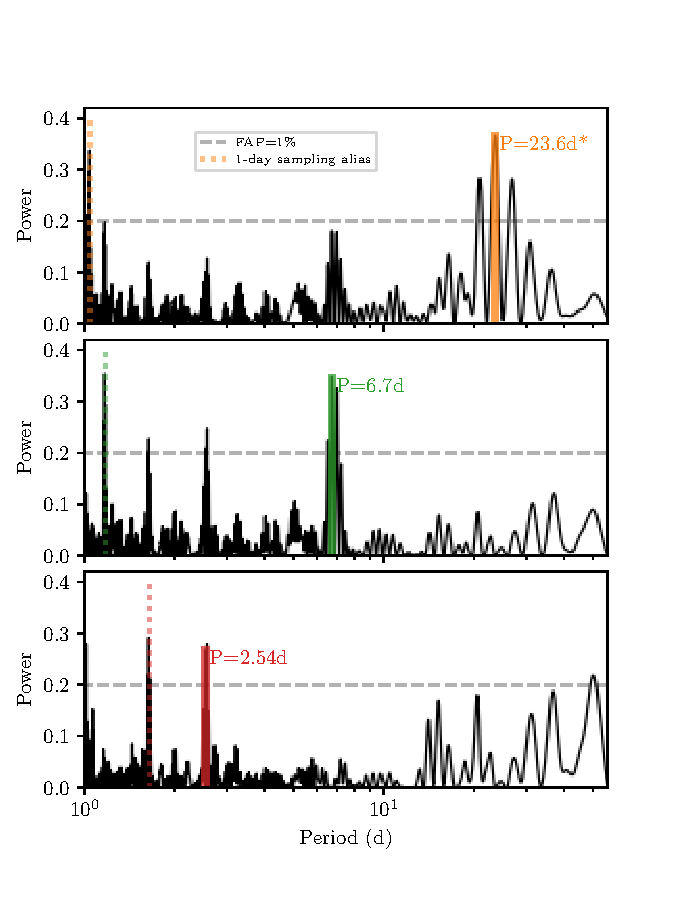
\includegraphics[width=\columnwidth, trim={0.3cm 1.1cm 0.8cm 1.3cm}]{TOI755_decorrelation_periodograms}
    \caption{Periodograms of RVs after linear decorrelation with S-index and FWHM. The upper panel shows the raw periodogram, while subsequent panels show the periodogram after the removal of the previously marked peak. The 2.54d peak is accompanied by a significant peak at the 1-day sampling alias (1.65d), but the knowledge of a 2.54d planet in the TESS photometry breaks this degeneracy.}
    \label{fig:rv_decorr}
\end{figure}
% \begin{figure}
% 	% To include a figure from a file named example.*
% 	% Allowable file formats are eps or ps if compiling using latex
% 	% or pdf, png, jpg if compiling using pdflatex
% 	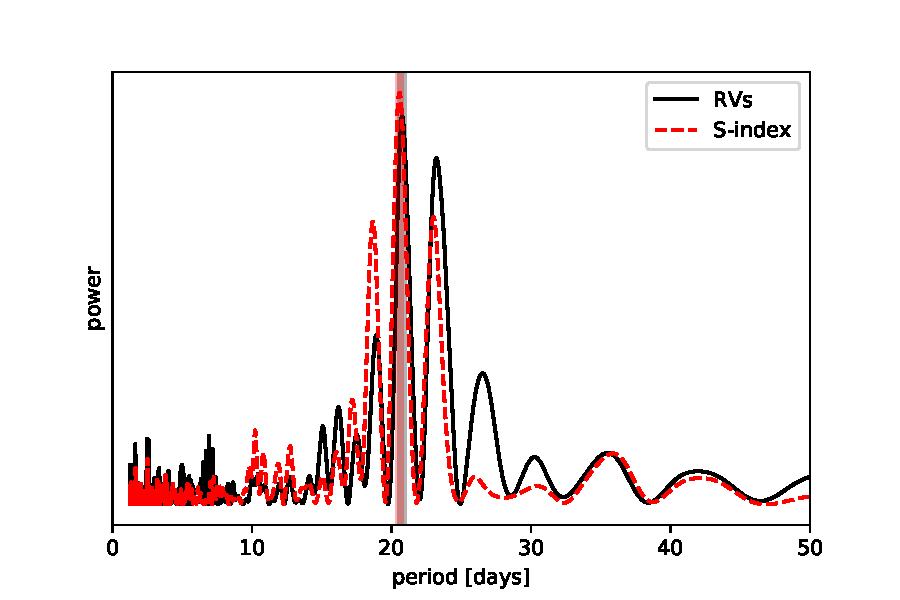
\includegraphics[width=\columnwidth]{LombScargle_755}
%     \caption{The Lomb-Scargle of both the S-index and RV. Overplotted in grey are the derived maximum signals which are in close agreement and suggest a rotation period of \TSindexperiod}
%     \label{fig:Sindex}
% \end{figure}

\begin{figure*}
	% To include a figure from a file named example.*
	% Allowable file formats are eps or ps if compiling using latex
	% or pdf, png, jpg if compiling using pdflatex
	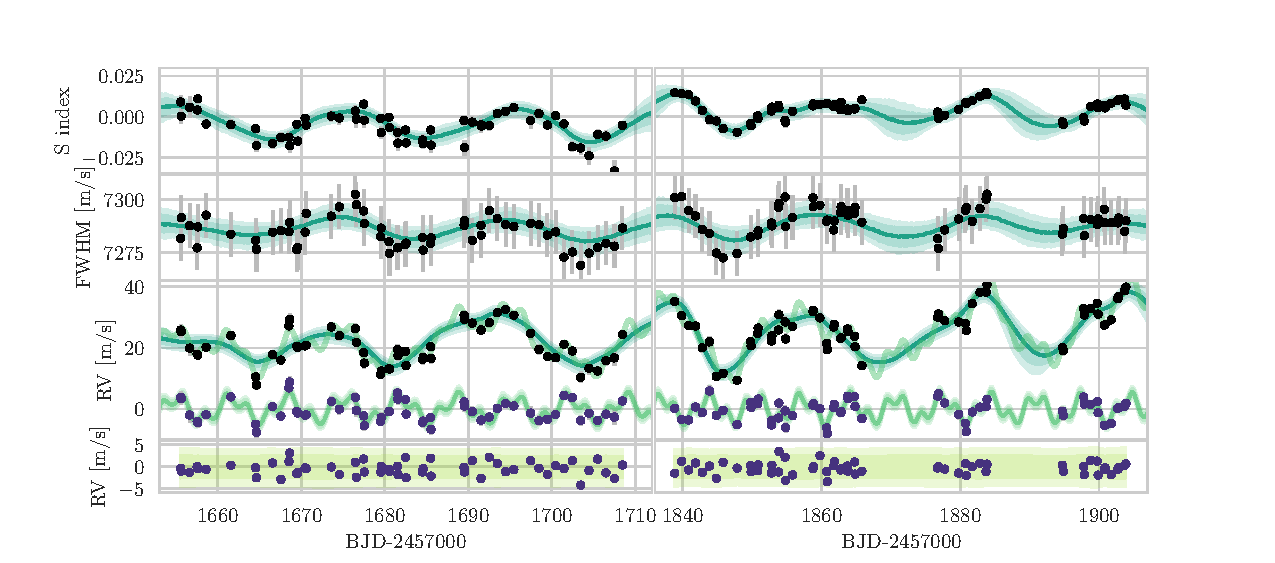
\includegraphics[width=\textwidth, trim={0.85cm 0.8 1.9cm 0.4cm}]{Combined_RV_plots_3_GPs.pdf}
    \caption{S-index, FWHM and RV timeseries, with GP models and 2-sigma uncertainty regions overplotted in green. Below the raw RV timeseries is the GP-removed timeseries showing the sum of the two planets models, and their uncertainties. At the very bottom the full model residuals are shown, with an RMS of only 1.50\ms{} only 0.11\ms{} above the average HARPS measurement uncertainties.}
    \label{fig:RVs}
\end{figure*}

\begin{figure}
	% To include a figure from a file named example.*
	% Allowable file formats are eps or ps if compiling using latex
	% or pdf, png, jpg if compiling using pdflatex
	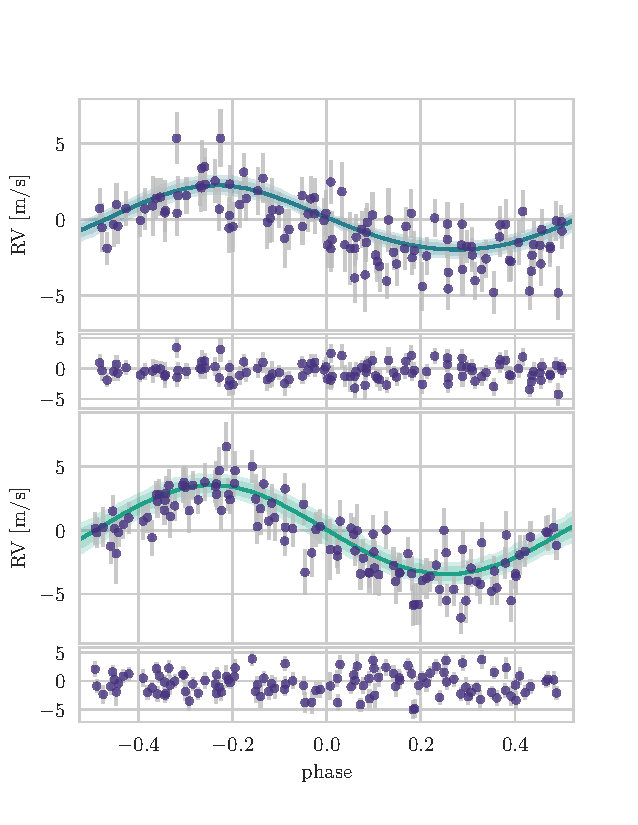
\includegraphics[width=\columnwidth, trim={0.1cm 0.8cm 1.0cm 0.85cm}]{Phase_folded_RV_plots_3_GPs}
    \caption{The phase-folded RV lightcurves for \Tplanet{} and \Tplanetc{}.}
    \label{fig:phase_fold_rvs}
\end{figure}

\subsubsection{Treatment of Photometry}
First, we normalised the \texttt{PDC\_SAP} timeseries and masked anomalous flux points from the timeseries by cutting data more than $4.2\sigma$ above both preceding and succeeding neighbours.

We initially tried to use the same \texttt{celerite} GP kernel to predict both RV and photometric time series deviations.
This proved to not be possible, likely because the effect of stellar variability on photometry is not necessarily at the same timescale as for RVs \citep{10.1111/j.1365-2966.2011.19960.x}.
Similarly, although a Lomb-Scargle periodogram of the raw TESS lightcurve does show a peak with a period around 25d, the processed \texttt{PDC\_SAP} lightcurve is flat, likely as variability on  the order of a TESS orbit ($\sim 14d$) are removed during processing.
Instead we used a separate, single-SHO kernel with quality $Q=1/\sqrt{2}$ to model the photometric stellar variability.
To produce the initial hyperparameters and priors for the combined analysis and reduce the possibility of the GPs attempting to model out the transits themselves, we first fitted this GP to the photometry with planetary transits cut. The interpolated posterior distributions from this analysis then provided the priors for the combined analysis.
A jitter term was also included to model the effect of high-frequency noise not fully encapsulated by the photon noise (e.g. stellar jitter).

We modelled the limb darkening using two approaches - one where limb darkening is fitted for for the data alone using the reparameterisation of \citet{kipping2013efficient}, and another where the theoretical limb darkening parameters for the star as generated by \citet{claret2017limb} are used as priors for the analysis.
We found the resulting distributions to be consistent, and chose to use the constrained approach in the final modelling.
Radius ratio $R_p/R_s$ was treated using the log amplitude to avoid negative values, and $R_p/R_s$ \& b were reparameterised following the \texttt{exoplanet} implementation of \citet{espinoza2018efficient}.

As ground-based photometry was unable to produce significant transit measurements, we restrict this analysis to only the \tess{} photometry and \harps{} spectroscopy.

\subsubsection{Combined Model}
We modelled full keplerian orbits for the two planets, with eccentricity priors according to the \citet{kipping2013parametrizing} beta distribution.

Monte Carlo sampling, while able to explore the parameter space around a best-fit solution, does not deal well with exploring unconstrained parameters with multiple local minima. 
This is specifically true with planetary period and epoch, especially in the case of the 6.7d planet which does not appear to have corresponding transit events. 
Therefore, in order to allow our model to explore a single solution, we included normal priors on period and $t_0$ using the values and uncertainties from the TOI catalogue in the case of the $2.54$d planet, and from the RV periodogram in the case of the $6.7$d planet.

The combined model, built using \textsf{exoplanet} \citep{exoplanet} package, was sampled using the No-U Turn Sampler (NUTS) in the Hamiltonian Monte Carlo \texttt{PyMC} back-end \citep{exoplanet:pymc3} to produce 3600 independent samples (after 500 steps tune-in).

The results from the combined model are shown in table \ref{table:datatable}, with the \harps{} RV timeseries and best-fit models shown in figure \ref{fig:RVs}, phase-folded RVs and model shown in figure \ref{fig:phase_fold_rvs}, and \tess{} photometry and best-fit light curves shown in figure \ref{fig:photometry}.

\begin{figure*}
	% To include a figure from a file named example.*
	% Allowable file formats are eps or ps if compiling using latex
	% or pdf, png, jpg if compiling using pdflatex
	%[left,bottom,right,top]
	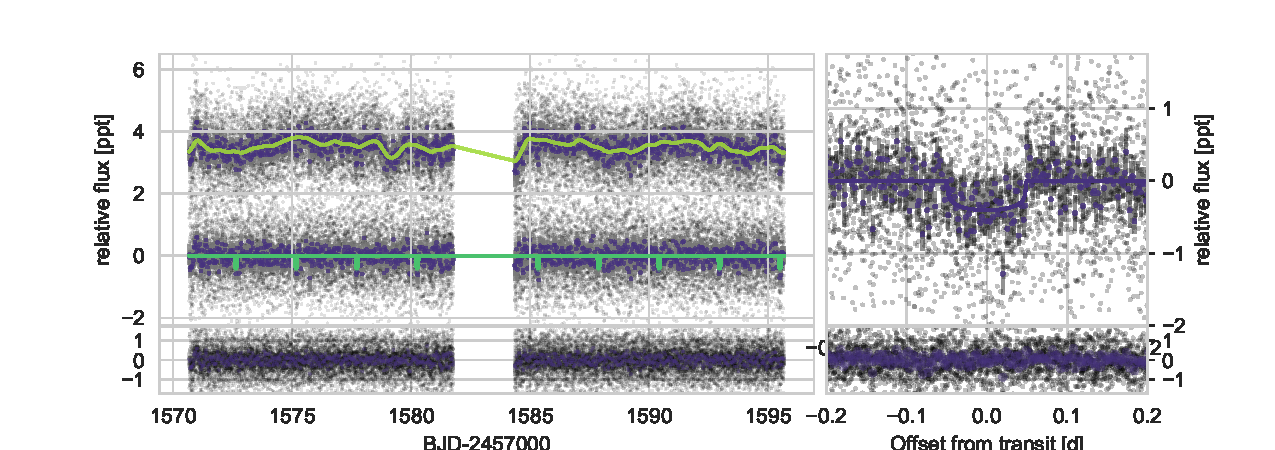
\includegraphics[width=\textwidth, trim={1.45cm 0.2 0.95cm 0.5}]{Combined_phot_plot_3_GPs}
    \caption{\tess{} photometry, where black dots represent individual 2-minute cadence data and dark circles (with errorbars) represent 30-minute bins. Upper left: \tess{} \texttt{PDC\_SAP} time series with best-fit GP model (both offset by 3.5ppt), and GP-subtracted lightcurve with the best-fit transit model over-plotted (no offset). Lower left: residuals, with both GP model and transit models subtracted from the lightcurve. Upper right: phase-folded lightcurve of \Tplanet{} zoomed to the transit. Lower right: phase-folded residuals. }
    \label{fig:photometry}
\end{figure*}

\subsection{Evidence for \Tplanetc{}}
The periodogram of the activity-corrected radial velocity timeseries showed a clear signal at $6.75$d, even stronger than that of the planet at $2.54$d (Figure \ref{fig:rv_decorr}).
Using the epoch and period defined from a fit to this decorrelated RV timeseries, we searched the TESS lightcurve to see whether a transiting planet on this period may have been missed.

However, a search using the \texttt{transit least squares} algorithm \citep{heller} on the model-subtracted lightcurve found no signal around 6.7d, and a visual inspection of the lightcurve around the likely epochs of transit reveals no candidate dips associated with an outer candidate.
Indeed, when running a combined model of two transiting planets, with constraints on orbits from the RVs, the posteriors for the radius of the outer planet were $0.05^{+0.59}_{−0.04}$\rearth{} which, given the \TMpone{}\mearth{} mass of \Tplanetc{}, would be physically impossible even with an iron-core.
Therefore we come to the conclusion that \Tplanetc{} is non-transiting.

In order to assess whether the RV signal alone warrants calling \Tplanetc{} a confirmed planet or merely a candidate, we ran two combined models with identical priors, and with one model including a non-transiting planet around $6.7$d.
We then burned in each model for 500 samples and ran the \texttt{find\_MAP} function in \texttt{PyMC3} to find the maximum likelihood for each model, allowing us to compare the difference in Bayesian Information Criterium ($\Delta{\rm BIC}$) between the models.
The resulting value of $\Delta{\rm BIC}= $\TdeltaBIC{} clearly favours a two-planet model over a single planet model, with $\Delta{\rm BIC}>10$ suggesting "Very Strong" evidence over the null hypothesis. 

It should be noted that the period of \Tplanetc{}, at \TPone{}d, is close to the $P_{\rm rot}/3$ harmonic.
However, there appears little evidence of a signal in the RV periodogram at $P_{\rm rot}/2$, so a large coherent signal at $P_{\rm rot}/3$ would be unexpected.
However, it is possible that with certain inclinations and spot locations such harmonics may be boosted \citep{vanderburg2016radial,boisse2011disentangling}.
Interestingly the periodogram of the S-index data does show a strong peak at $P_{\rm rot}/2$ and a weaker peak at $P_{\rm rot}/3$, but this occurs at $7.25$d - significantly separated from the RV peak at \TPone{}.
Even if a real candidate, as our $\Delta{\rm BIC}>10$ suggests, the amplitude of the signal may be impacted by the presence of a signal at $P_{\rm rot}/3$, therefore the mass of \Tplanetc{} should be treated as uncertain. 

However, multiple lines of evidence point to the candidate signal of \Tplanetc{} being planetary in origin.
Future RV measurements should help further disentangle stellar rotation and the signal amplitude, and may even reveal new candidates in this system.

The majority of short-period multi-planet systems have low mutual inclinations \citep{lissauer2011architecture}, and in such a case the non-transiting nature of \Tplanetc{} is not unexpected.
Using the derived impact parameter of planet $b$ and the semi-major axis of $c$, the expected impact parameter of planet c is $0.8\pm0.4$ producing a non-transiting planet in $32\%$ of scenarios.
It is also worth noting that planets b \& c have an orbital period ratio near 8/3, although harmonics beyond $2:1$ are highly unlikely to create measurable TTVs \citep{deck2015measurement}.

\section{Discussion}
\subsection{Composition}
Jon's results.

If gas-rich ~1\% by-mass and 50\% by volume.

\subsection{Evaporation}
Using Prot = 21d with Wright+18; Lx/Lbol = 8.5e-7; Lx = 3.3e27 erg; current mass loss rate is 5.0e9 g/s.

Using age = 3Gyr with Jackson+12; Lx/Lbol = 2.74e-6; Lx = 1.05e28 erg; current mass loss rate is 9.9e9 g/s (0.026\% per Gyr).
If, as you opined, the star is a bit older, Lx and the mass loss rate should drop to closer to the value from the rotation.

These mass loss rates assume the energy limited method. This is comparable, maybe a bit higher than both GJ 436b and Pi Men c under similar assumptions.

Again assuming a 3 Gyr lifetime with the X-ray-age evolution of Jackson+12. As I said before, this also assumes a constant radius, which in reality there will be changes as mass is lost.


Starting at the current mass and radius -> 9.7\% lost.

Neptune mass and radius with the same irradiation history as TOI-755b -> 5.4% lost

Jupiter mass and radius with the same irradiation history as TOI-755b -> 0.41%

It is almost certain that \Tplanet{} started with a thicker atmosphere of H/He, which due to both evaporative and core-powered mass-loss, it lost much of over time.
The main unanswered question is therefore: how did \Tplanet{} escape becoming a naked core devoid of light elements?

Due to the degeneracies in the planets composition, there exists two solutions:
The first is that \Tplanet{} started with a large quantity of H-He, perhaps as much as 10\%, which was gradually lost to evaporation and core-powered heating over time, but it started with enough gaseous 
Two possibilities - our planet had an evaporative history that precisely matched the decrease in x-ray luminosity of the star, allowing it to maintain a small H2-He layer until late ages..
Our planet lost all its H-He early on and is instead a water-rich ice-giant.

\subsection{Re-observation}
Even with the detection of TTVs caused by \Tplanetc{} appearing unlikely, \Tplanet{} may benefit from further observations.
\Tplanet will be re-observed by \tess{} during Sector 37\footnote{\url{https://heasarc.gsfc.nasa.gov/cgi-bin/tess/webtess/wtv.py?Entry=73228647}}, and could be observed by ESA's \textit{Cheops} telescope \citep{benz2020cheops}, both of which would improve the current radius error below the currently measured value of 7\%, thereby improving our knowledge of the internal structure of \Tplanet{}.

The low-density nature and bright stellar magnitude of this hot mini-Neptune may enable transmission spectroscopy.


%
%\begin{table*}[t]
%    \centering
%    \caption{
%    }
%    \begin{tabular}{cc|cc}
%    \hline
%    \hline
%    \multicolumn{2}{l}{Catalogue data} & \multicolumn{2}{l}{Model parameters}     \\
%    \hline
%%Gaia Source ID & \TGAIAid        & $T_0$ (BJD-TDB) & \TfitTO  \\
%TIC ID & \TICstar        & $T_0$ (BJD-TDB) & \Ttzerozero  \\
%R.A.  &  \Tstarra      & $P$ (d) &  \TP \\
%decl.  & \Tstardec     & $b$  & \Tb \\
%G & \TGAIAGmag         & $u_{\rm TESS}(0)$ & \Tuzero \\
%%BP & \TGAIABPmag                 & $b$          & \Tfitb \\
%%RP & \TGAIARPmag                &  $h_{1,\rm \tess}$  & \TfithItess  \\
%pmRA (\masy)   & \TGAIAPMRA  & $u_{\rm TESS}(1)$ & \Tuone \\
%pmDec (\masy)  & \TGAIAPMDec &  $K_\star$ (\kms) & \TlogK \\
%Parallax ($\rm mas$) & \TGAIAplx 
%\tess\ (T)   & \TESSTmag 
%% APASS9 (B) & \APASSBmag 
%% APASS9 (V) & \APASSVmag & $\sqrt{e}\sin \omega$ & \Tfitfs  \\
%% APASS9 (g') & \APASSgmag & $\sqrt{e}\cos \omega$& \Tfitfc  \\
%% APASS9 (r') & \APASSrmag &  $\gamma$ (\kms)& \TfitV \\ 
%% APASS9 (i') &\APASSimag & $\Delta \gamma_{\rm FEROS}$ (\kms)& \TfitHF\\
%\cline{3-4}
%2MASS (J)  & \MASSJ  &  \multicolumn{2}{l}{Derived planet properties} \\
%\cline{3-4}
%2MASS (H)  & \MASSH  & \mpl\ (\mjup) & \Tplanetmass \\
%2MASS (K$_{\rm s}$)& \MASSK &  \rpl\ (\rjup) &  \Tplanetradius  \\
%\cline{1-2}
%\multicolumn{2}{l|}{Stellar parameters} &  $a\,(\rm au)$ & \Tpa \\  
%\cline{1-2}
%\teff\ (K) &  \Tteff & e & \Tfite   \\
%\feh\ ($\rm dex$) &  \TFeH &  $\omega$ (deg) & \Tfitw \\  
%$\log g_\star$ ($\rm dex$) &  \Tlogg &  $i$ (deg) & \Tpincl  \\
%%\vsini\ (\kms) & \Trotation  &  $T_{\rm dur}$ (hr) & \Tfitdur \\
%\mstar\ (\msun) &  \TMs  & $g_p$ (\mss)& \Tpgrav\\
%\rstar\ (\rsun) & \TRs  & $T_{\rm eq}$ $(\rm K)$ & \Teq  \\
%%$\rho_\star$\ ($\rho_{\sun}$) & \Tstardensity & $\rho_{p}$\ (g\,cm$^{-3}$) & \Tpden  \\
%%Age $(\rm Gyr)$ & \Tstarage & $H_p$ (km)& \TpH \\
%\hline
%    \end{tabular}
%    \label{table:datatable}
%\end{table*}

% \begin{figure*}
% \makebox[\textwidth][c]{
%  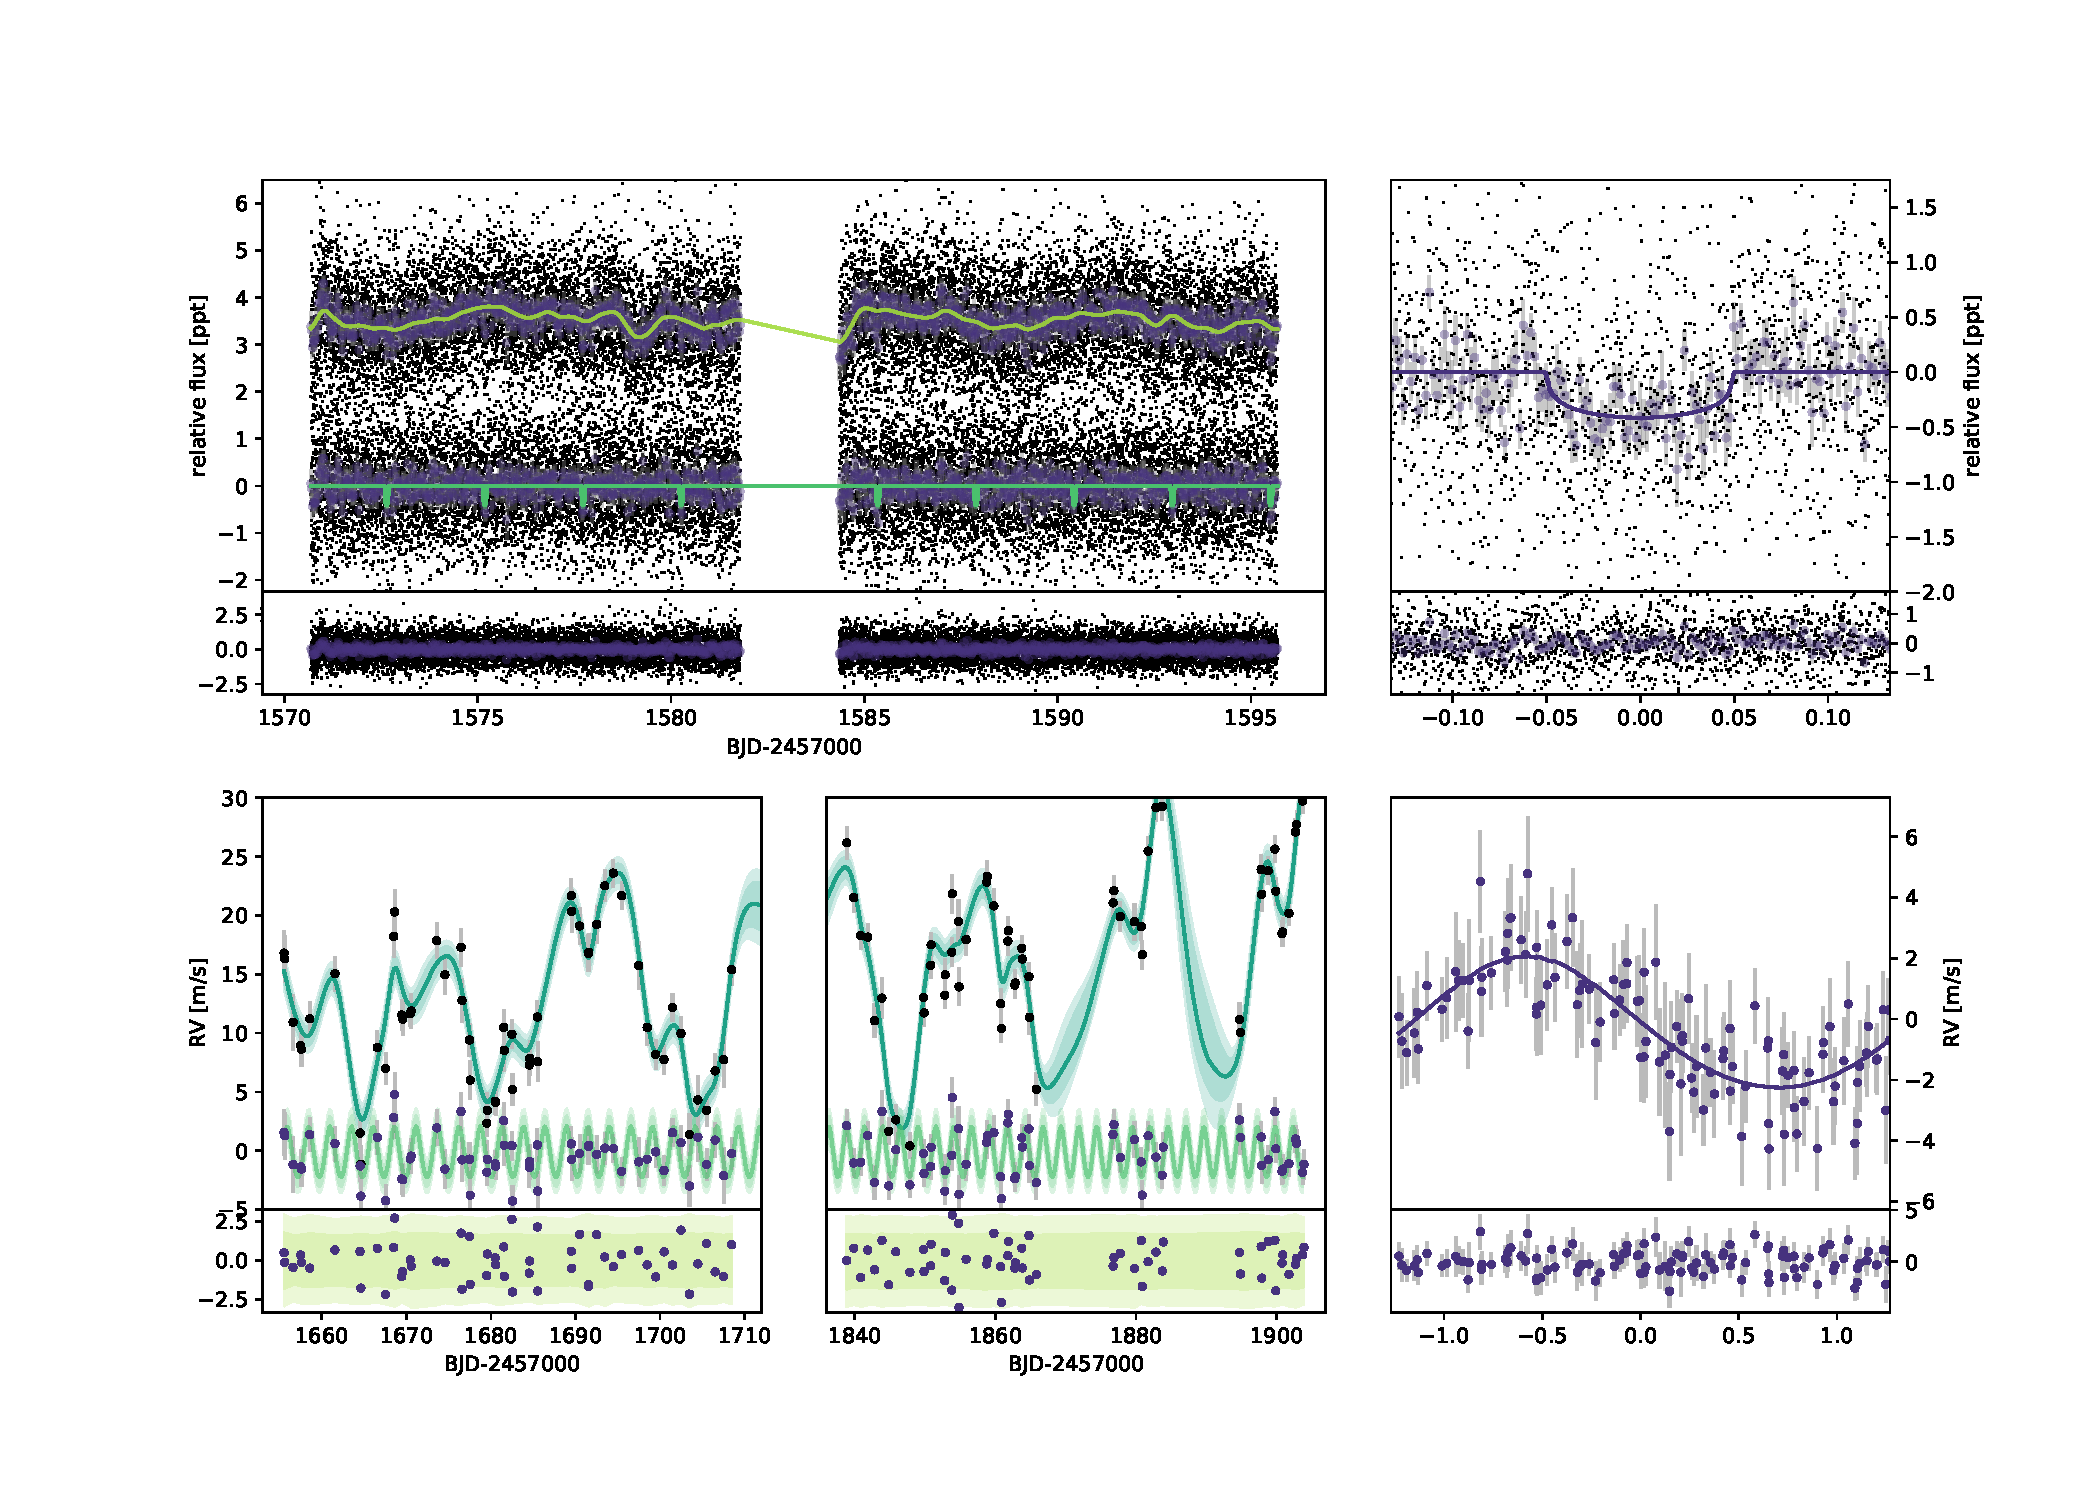
\includegraphics[width=\paperwidth]{Combined_Model_plots_2xGP_smooth}
% }
% \caption{Photometric \& RV time series.
% Detrended \tess Lightcurve both with and without best-fit Gaussian Process; transit model lightcurve residuals after subtraction of GP and transit model (centre left);
% Phase-folded lightcurve centred on transit with best-fit model (upper right); Phase-folded model residuals (centre right);
% Detrended \harps RVs both with and without S-index-trained Gaussian Process model (lower left); 
% RV residual time series after subtraction of GP and planet model (bottom left);
% Phase-folded RVs with best-fit RV model (lower right); Phase-folded RV residuals (bottom right).
% }
% \label{FullTransitFits0}
% \end{figure*}

\section{Conclusion}


\begin{figure}
	% To include a figure from a file named example.*
	% Allowable file formats are eps or ps if compiling using latex
	% or pdf, png, jpg if compiling using pdflatex
	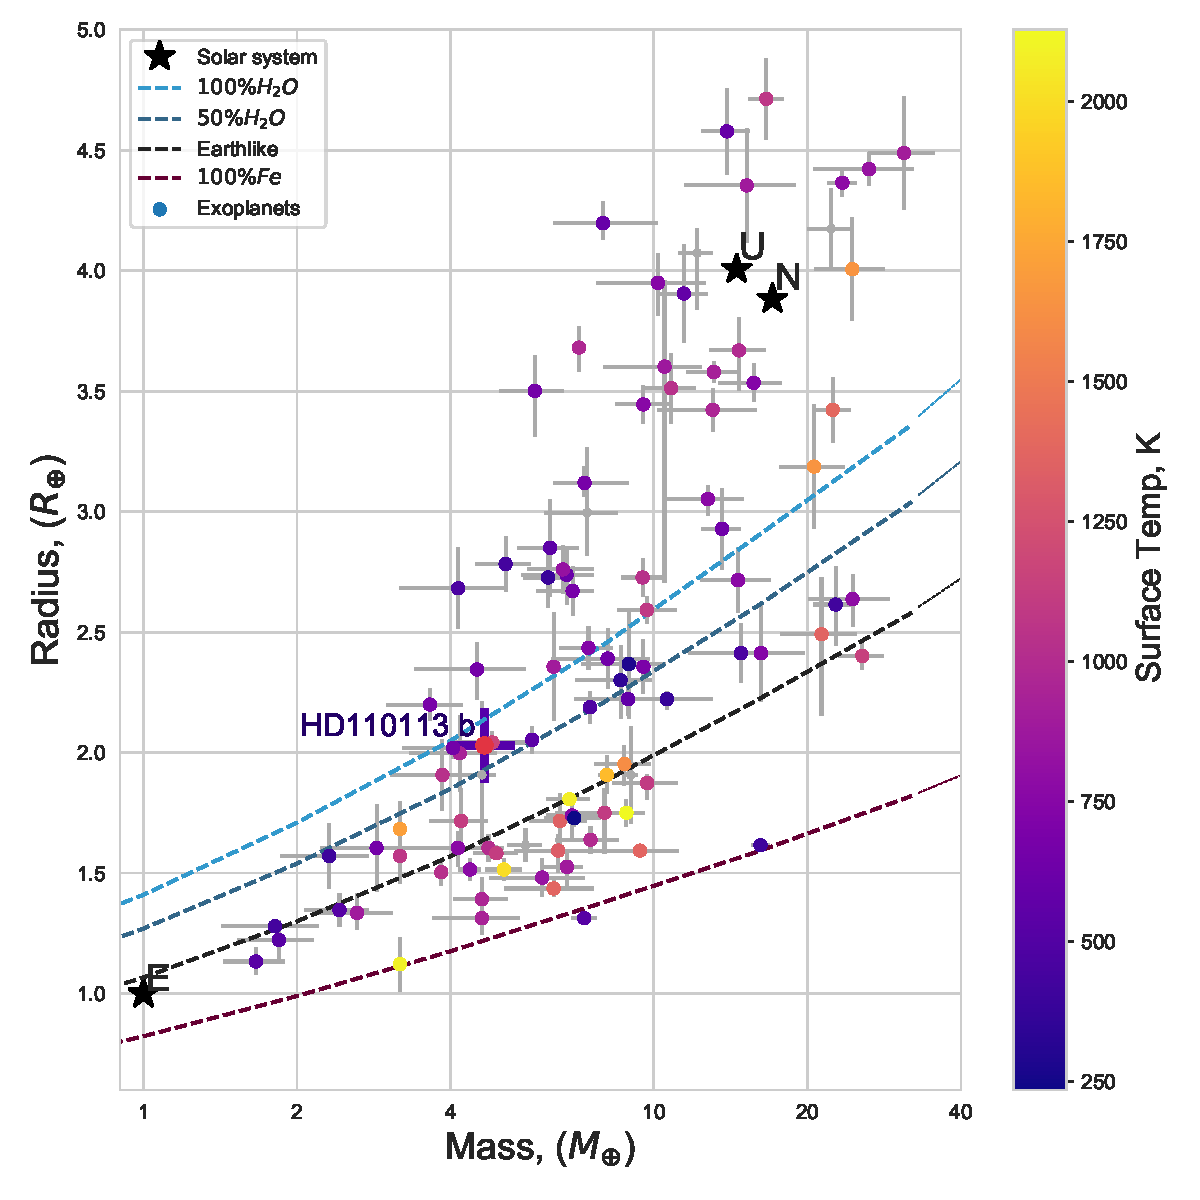
\includegraphics[width=\columnwidth]{MR_Diagram_sm}
    \caption{A Mass-Radius diagram for small planets with masses and radii constrained to better than SNR=4, with data from the NASA exoplanet archive \citep{akeson2013nasa}. Colour coding shows the surface temperature of each planet (assuming an albedo of 0.2). Solar System planets are marked with stars.}
    \label{fig:example_figure}
\end{figure}

% Example table
\begin{table}
	\centering
	\caption{Derived planet properties.}
	\label{tab:derived_pars}
\begin{tabular}{lcc}
\hline
\hline
Parameter & b & c\\
\hline
\hline
Epoch, $t_0$ [BJD-2457000] &  $ 1570.1006 \pm 0.0044 $  &  $ 1798.18 \pm 0.18 $  \\
Orbital Period, $P$ [d] &  $ 2.5408 \pm 0.00049 $  &  $ 6.744^{+0.0084}_{-0.0085} $  \\
Semi-major Axis, $a$ [AU] &  $ 0.03755 \pm 0.00093 $  &  $ 0.06979 \pm 0.00023 $  \\
Orbital Eccentricity, $e$ &  $ 0.102^{+0.088}_{-0.068} $  &  $ 0.05^{+0.076}_{-0.037} $  \\
Argument of periasteron, $\Omega$ &  $ -0.35^{+0.99}_{-0.8} $  &  $ 0.8 \pm 1.1 $  \\
Radius ratio [$R_p/R_s$] &  $ 0.0196 \pm 0.0013 $  & --- \\
Radius, $R_p$ [$R_\oplus$] &  $ 2.08 \pm 0.13 $  & --- \\
Impact Parameter, b &  $ 0.46^{+0.17}_{-0.25} $  & --- \\
Transit duration, $t_D$ [d] &  $ 0.0992^{+0.0055}_{-0.0067} $  & --- \\
RV semi-amplitude, $K$ [\ms{}] &  $ 2.14 \pm 0.28 $  &  $ 3.57 \pm 0.39 $  \\
Planet Mass, $M_p$ [$M_\oplus$] &  $ 4.51 \pm 0.6 $  &  $ 10.5 \pm 1.1 $  \\
Planet Density, $\rho_p$ [${\rm gcm}^{-3}$] &  $ 2.77^{+0.69}_{-0.57} $  & --- \\
Insolation, $S$ [${\rm Wm}^{-2}$] &  $ 1001000^{+7900}_{-7300} $  &  $ 290000 \pm 15000 $  \\
Surface Temperature, $T_p$ [K] &  $ 1370.8^{+2.7}_{-2.5} $  &  $ 1006.0 \pm 13.0 $  \\
\hline
\hline
\end{tabular}
\end{table}

\onecolumn
\centering
\begin{table*}
\caption{List of free parameters used in the \texttt{exoplanet} combined analysis of the \tess{} light curve and \harps{} radial velocities with their associated prior and posterior distributions.}
\label{tab:planetparlong}
\begin{center}
\begin{tabular}{lcc}
\hline
\hline
Parameter & Prior & Posterior\\
\hline
\hline
\multicolumn{3}{l}{\it Stellar parameters}\\
Stellar surface temperature, \teff{} [K] &  $\mathcal{N}(5732.0,16.0)$  &   $ 5734.1^{+5.7}_{-3.9} $ \\
Stellar Mass, $M_s$ [$M_{\odot}$] &  $\mathcal{N}(0.9968,0.0095)$  &   $ 0.997^{+0.0098}_{-0.0094} $ \\
Stellar Radius, $R_s$ [$R_{\odot}$] &  $\mathcal{N}(1.0348,0.0256)$  &   $ 1.032 \pm 0.025 $ \\
\hline
\multicolumn{3}{l}{\it Orbital parameters}\\
Transit Epoch, $t_0$ [BJD-2457000] b &  $\mathcal{N}(1570.10189,0.1)$  &   $ 1570.1006 \pm 0.0044 $ \\
Transit Epoch, $t_0$ [BJD-2457000] c &  $\mathcal{N}(1798.1334,1.0)$  &   $ 1798.18 \pm 0.18 $ \\
Orbital Period, $P$ [d] b &  $\mathcal{N}_{\mathcal{U}}(2.540455,0.002124,2.35,2.6)$  &   $ 2.5408 \pm 0.00049 $ \\
Orbital Period, $P$ [d] c &  $\mathcal{N}_{\mathcal{U}}(6.7285,0.05951,6.65,6.8)$  &   $ 6.744^{+0.0084}_{-0.0085} $ \\
Orbital Eccentricity, $e$ b &  $\beta(0.867;3.03)^{\tnote{a}}$  &   $ 0.102^{+0.088}_{-0.068} $ \\
Orbital Eccentricity, $e$ c &  $\beta(0.867;3.03)^{\tnote{a}}$  &   $ 0.05^{+0.076}_{-0.037} $ \\
Argument of periasteron, $\Omega$ b &  $\mathcal{U}(-\pi,\pi)^{\tnote{b}}$  &   $ -0.35^{+0.99}_{-0.8} $ \\
Argument of periasteron, $\Omega$ c &  $\mathcal{U}(-\pi,\pi)^{\tnote{b}}$  &   $ 0.8 \pm 1.1 $ \\
\hline
\multicolumn{3}{l}{\it Photometric parameters}\\
log radius ratio [$\log{R_p/R_s}$] b &  $\mathcal{U}(-11.513,-2.3023)$  &   $ -3.932 \pm 0.067 $ \\
Transit Impact Parameter b & $\mathcal{U}(0,1+R_p/R_s)^{\tnote{c}}$  &   $ 0.46^{+0.17}_{-0.25} $ \\
Quadratic Limb Darkening $a_{\rm LD}$ &  $\mathcal{N}_{\mathcal{U}}(0.367,0.1,0.0,1.0)$  &   $ 0.38 \pm 0.1 $ \\
Quadratic Limb Darkening $b_{\rm LD}$ &  $\mathcal{N}_{\mathcal{U}}(0.21,0.1,0.0,1.0)$  &   $ 0.208 \pm 0.097 $ \\
Photometric jitter [$\log{\rm ppt}$] &  $\mathcal{N}(0.7294,5.0)$  &   $ -7.7^{+1.4}_{-2.1} $ \\
Photometric GP power & $\mathcal{I}{0.014,0.006}^{\tnote{d}}$  &   $ 0.0116^{+0.0033}_{-0.0025} $ \\
Photometric GP frequency [$d^{-1}$] & $\mathcal{I}{3.525,0.651}^{\tnote{d}}$  &   $ 3.79^{+0.46}_{-0.43} $ \\
Photometric GP mean [ppt] & $\mathcal{I}{0.008,0.036}^{\tnote{d}}$  &   $ 0.012^{+0.035}_{-0.036} $ \\
\hline
\multicolumn{3}{l}{\harps{} parameters}\\
log RV semi-amplitude, $\log{K}$ b &  $\mathcal{N}(0.3,5.0)$  &   $ 0.76 \pm 0.13 $ \\
log RV semi-amplitude, $\log{K}$ c &  $\mathcal{N}(0.3,5.0)$  &   $ 1.27 \pm 0.11 $ \\
RV trend - intercept at BJD=2458779.717 [\ms{}] &  $\mathcal{N}(0.0,0.1)$  &   $ 0.027 \pm 0.01 $ \\
RV trend - gradient [\ms{}$d^{-1}$] &  $\mathcal{N}(0.0,1.0)$  &   $ -0.14 \pm 0.73 $ \\
\harps{} log jitter RV [\ms{}] &  $\mathcal{N}(1.992,5.0)$  &   $ -0.9^{+1.0}_{-3.9} $ \\
\harps{} log jitter S index &  $\mathcal{N}(6.527e-06,5.0)$  &   $ -13.0 \pm 0.8 $ \\
\harps{} log jitter FWHM [\ms{}] &  $\mathcal{N}(20.525,5.0)$  &   $ -0.2 \pm 1.2 $ \\
\harps{} mean S-index &  $\mathcal{N}(0.0,0.00941)$  &   $ -0.0002 \pm 0.0014 $ \\
\harps{} mean FWHM [\ms{}] &  $\mathcal{N}(7287.75,7.5)$  &   $ 7287.0 \pm 1.2 $ \\
\harps{} GP log amplitude RV &  $\mathcal{N}(2.984,8.0)$  &   $ 3.69 \pm 0.33 $ \\
\harps{} GP log amplitude S-index &  $\mathcal{N}(-9.332,8.0)$  &   $ -9.63 \pm 0.33 $ \\
\harps{} GP log amplitude FWHM &  $\mathcal{N}(4.03,8.0)$  &   $ 3.76^{+0.37}_{-0.35} $ \\
\harps{} GP log rotation period, $\log{P_{\rm rot}}/\log{d}$ &  $\mathcal{N}_{\mathcal{U}}(3.024,0.2,1.099,4.382)$  &   $ 3.028 \pm 0.06 $ \\
\harps{} GP log quality, $Q$ &  $\mathcal{N}(0.0,10.0)$  &   $ -3.2^{+3.4}_{-4.0} $ \\
\harps{} GP log quality differential, $\delta Q$ &  $\mathcal{N}(0.0,5.0)$  &   $ 0.6 \pm 0.9 $ \\
\harps{} GP $P_{\rm rot}$ - $P_{\rm rot}/2$ mix factor &  $\mathcal{U}(0,1)$  &   $ 0.033^{+0.053}_{-0.022} $ \\
\hline
\hline
\multicolumn{3}{l}{%
  \begin{minipage}{14cm}%
    $\mathcal{N}(\mu;\sigma^{2})$ is a normal distribution with mean $\mu$ and width $\sigma^{2}$, $\mathcal{U}(a;b)$ is a uniform distribution between $a$ and $b$, $\mathcal{N}_{\mathcal{U}}(\mu;\sigma^{2},a,b)$ is a normal distribution with mean $\mu$ and width $\sigma^{2}$ multiplied with a uniform distribution between $a$ and $b$, $\beta(a;b)$ is a Beta distribution with parameters $a$ and $b$, and $\mathcal{I}(\mu;\sigma^2)$ is a distribution directly interpolated from the output of a pre-trained distribution with mean $\mu$ and standard deviation $\sigma^2$.  Posterior values and uncertainties represent the median and $1\sigma$ error boundaries. All other values (e.g. presented in Table \ref{tab:derived_pars}) are directly determined from these fitted quantities. $^{\tnote{a}}$Described in \citet{kipping2013parametrizing}.  $^{\tnote{b}}$Reparameterised in \texttt{exoplanet} to avoid discontinuities at $\pm\pi$. $^{\tnote{c}}$\texttt{exoplanet} reparameterization of \citet{espinoza2018efficient}. $^{\tnote{d}}$\texttt{PyMc3} Interpolation function of pre-trained GP.
  \end{minipage}%
}\\
\end{tabular}
\tablefoot{
\end{center}
\label{AllPriors}
\end{table*}%
\twocolumn

\begin{table}
\caption{\harps{} spectroscopy from first season (June - August 2019)}
\label{Spec1}
\small
\begin{tabular}{lccc}
\hline
\hline
Time & RV [\ms{}] & $S_{\rm MW}$ & FWHM [\ms{}] \\
\hline
\hline
$1655.5493$ & $1.8\pm1.95$ & $0.0091\pm0.004$ & $7281.8\pm10.3$ \\
$1655.6181$ & $1.32\pm2.0$ & $0.0003\pm0.0045$ & $7291.5\pm10.4$ \\
$1656.6167$ & $-4.08\pm2.39$ & $0.0059\pm0.0064$ & $7287.6\pm10.4$ \\
$1657.5254$ & $-6.07\pm1.44$ & $0.0042\pm0.0025$ & $7277.2\pm10.4$ \\
$1657.606$ & $-6.37\pm1.49$ & $0.011\pm0.0029$ & $7287.2\pm10.4$ \\
$1658.5953$ & $-3.78\pm1.46$ & $-0.0045\pm0.0031$ & $7292.7\pm10.4$ \\
$1661.5662$ & $0.04\pm1.48$ & $-0.0048\pm0.003$ & $7283.7\pm10.4$ \\
$1664.5324$ & $-13.5\pm1.36$ & $-0.0074\pm0.0028$ & $7280.8\pm10.4$ \\
$1664.6282$ & $-16.17\pm1.6$ & $-0.0177\pm0.004$ & $7276.6\pm10.4$ \\
$1666.5674$ & $-6.22\pm1.45$ & $-0.0164\pm0.0029$ & $7284.6\pm10.4$ \\
$1667.5542$ & $-8.01\pm1.39$ & $-0.0127\pm0.0028$ & $7285.4\pm10.4$ \\
$1668.5189$ & $3.21\pm1.8$ & $-0.0126\pm0.0036$ & $7284.8\pm10.3$ \\
$1668.6197$ & $5.3\pm1.88$ & $-0.0178\pm0.0044$ & $7289.2\pm10.4$ \\
$1669.466$ & $-3.47\pm1.32$ & $-0.0046\pm0.0021$ & $7276.4\pm10.3$ \\
$1669.5709$ & $-3.81\pm1.42$ & $-0.015\pm0.0026$ & $7277.4\pm10.4$ \\
$1670.4637$ & $-3.35\pm1.13$ & $-0.0009\pm0.0015$ & $7284.6\pm10.4$ \\
$1670.5832$ & $-3.13\pm1.46$ & $-0.0052\pm0.0028$ & $7293.5\pm10.4$ \\
$1673.5985$ & $2.86\pm1.53$ & $0.0004\pm0.0032$ & $7292.2\pm10.4$ \\
$1674.5613$ & $-0.04\pm1.69$ & $-0.0008\pm0.0038$ & $7296.6\pm10.4$ \\
$1676.4716$ & $2.3\pm1.62$ & $0.0035\pm0.0034$ & $7302.6\pm10.4$ \\
$1676.5886$ & $-2.22\pm1.88$ & $-0.0014\pm0.0051$ & $7297.6\pm10.4$ \\
$1677.4681$ & $-5.59\pm1.43$ & $0.0078\pm0.0029$ & $7294.7\pm10.4$ \\
$1677.5491$ & $-9.0\pm1.68$ & $-0.0021\pm0.0043$ & $7288.7\pm10.4$ \\
$1679.5086$ & $-12.66\pm1.12$ & $-0.001\pm0.0019$ & $7282.5\pm10.4$ \\
$1679.571$ & $-11.58\pm1.56$ & $-0.0098\pm0.0036$ & $7286.5\pm10.4$ \\
$1680.5087$ & $-10.82\pm1.09$ & $-0.0003\pm0.0017$ & $7280.1\pm10.4$ \\
$1680.5634$ & $-10.88\pm1.16$ & $-0.0066\pm0.0021$ & $7274.6\pm10.4$ \\
$1681.5245$ & $-4.52\pm1.54$ & $-0.0098\pm0.0035$ & $7277.2\pm10.4$ \\
$1681.5771$ & $-6.48\pm1.75$ & $-0.0162\pm0.0043$ & $7277.4\pm10.4$ \\
$1682.4813$ & $-5.11\pm1.23$ & $-0.0081\pm0.002$ & $7278.9\pm10.4$ \\
$1682.5533$ & $-9.81\pm1.35$ & $-0.016\pm0.0028$ & $7279.4\pm10.4$ \\
$1684.5367$ & $-7.71\pm1.75$ & $-0.0143\pm0.0037$ & $7282.2\pm10.4$ \\
$1684.5971$ & $-7.15\pm1.49$ & $-0.0165\pm0.0031$ & $7276.2\pm10.4$ \\
$1685.4972$ & $-3.64\pm1.39$ & $-0.0081\pm0.003$ & $7279.2\pm10.4$ \\
$1685.5436$ & $-7.43\pm1.69$ & $-0.0174\pm0.0044$ & $7281.9\pm10.4$ \\
$1689.5056$ & $6.68\pm1.47$ & $-0.0023\pm0.0032$ & $7287.8\pm10.4$ \\
$1689.5493$ & $5.35\pm1.83$ & $-0.019\pm0.0047$ & $7290.2\pm10.4$ \\
$1690.4858$ & $4.11\pm1.6$ & $-0.0033\pm0.0032$ & $7280.8\pm10.3$ \\
$1691.5335$ & $1.79\pm1.58$ & $-0.005\pm0.0037$ & $7287.9\pm10.4$ \\
$1691.5549$ & $1.87\pm1.62$ & $-0.0057\pm0.0039$ & $7283.2\pm10.4$ \\
$1692.5178$ & $4.23\pm1.59$ & $-0.0053\pm0.0032$ & $7294.8\pm10.3$ \\
$1693.4664$ & $7.52\pm1.36$ & $0.002\pm0.0026$ & $7291.0\pm10.3$ \\
$1694.4709$ & $8.59\pm1.19$ & $0.0034\pm0.002$ & $7288.2\pm10.3$ \\
$1695.462$ & $6.68\pm1.21$ & $0.0056\pm0.0018$ & $7287.3\pm10.3$ \\
$1697.4761$ & $0.74\pm2.07$ & $-0.0023\pm0.0052$ & $7288.8\pm10.3$ \\
$1698.4702$ & $-4.52\pm1.57$ & $0.0019\pm0.0029$ & $7288.1\pm10.3$ \\
$1699.4797$ & $-6.82\pm1.3$ & $-0.0051\pm0.0024$ & $7283.2\pm10.3$ \\
$1700.4668$ & $-7.25\pm1.29$ & $0.0007\pm0.0023$ & $7284.8\pm10.3$ \\
$1701.4669$ & $-2.83\pm1.19$ & $-0.0044\pm0.0021$ & $7272.8\pm10.3$ \\
$1702.4715$ & $-5.04\pm1.47$ & $-0.0185\pm0.0032$ & $7275.2\pm10.3$ \\
$1703.4744$ & $-13.62\pm1.76$ & $-0.0192\pm0.0042$ & $7269.0\pm10.3$ \\
$1704.4713$ & $-10.69\pm2.09$ & $-0.024\pm0.0054$ & $7274.8\pm10.3$ \\
$1705.4964$ & $-11.55\pm1.38$ & $-0.0108\pm0.0029$ & $7277.4\pm10.3$ \\
$1706.4982$ & $-8.22\pm1.47$ & $-0.0119\pm0.0033$ & $7279.4\pm10.3$ \\
$1707.5135$ & $-7.27\pm2.37$ & $-0.0333\pm0.0066$ & $7278.0\pm10.3$ \\
$1708.4678$ & $0.39\pm1.35$ & $-0.0052\pm0.0026$ & $7286.6\pm10.3$ \\
\hline
\hline
\end{tabular}
\end{table}
\begin{table}
\caption{\harps{} spectroscopy from second season (Dec 2019 - Feb 2020).}
\label{Spec2}
\small
\begin{tabular}{lccc}
\hline
\hline
Time & RV [\ms{}] & $S_{\rm MW}$ & FWHM [\ms{}] \\
\hline
\hline
$1838.8494$ & $11.17\pm1.4$ & $0.0147\pm0.0022$ & $7301.0\pm10.3$ \\
$1839.8578$ & $6.52\pm1.26$ & $0.0142\pm0.0017$ & $7301.5\pm10.3$ \\
$1840.8432$ & $3.27\pm1.15$ & $0.0136\pm0.0014$ & $7294.8\pm10.3$ \\
$1841.8384$ & $3.16\pm1.19$ & $0.0097\pm0.0015$ & $7292.3\pm10.3$ \\
$1842.8077$ & $-3.96\pm1.45$ & $0.0039\pm0.0022$ & $7286.0\pm10.3$ \\
$1843.8559$ & $-2.03\pm1.74$ & $-0.0018\pm0.0029$ & $7284.0\pm10.3$ \\
$1844.8362$ & $-13.35\pm1.16$ & $-0.0026\pm0.0014$ & $7274.8\pm10.3$ \\
$1845.8271$ & $-12.38\pm1.33$ & $-0.0073\pm0.002$ & $7272.5\pm10.3$ \\
$1847.8389$ & $-14.59\pm1.11$ & $-0.0095\pm0.0012$ & $7274.5\pm10.3$ \\
$1849.7822$ & $-1.97\pm1.18$ & $-0.0042\pm0.0015$ & $7282.3\pm10.3$ \\
$1849.8576$ & $-3.28\pm1.13$ & $-0.0055\pm0.0013$ & $7282.4\pm10.3$ \\
$1850.7988$ & $0.75\pm1.08$ & $0.0006\pm0.0013$ & $7283.3\pm10.3$ \\
$1850.8597$ & $2.51\pm1.04$ & $-0.001\pm0.0011$ & $7285.2\pm10.3$ \\
$1852.7908$ & $-1.78\pm1.17$ & $0.0036\pm0.0015$ & $7289.0\pm10.3$ \\
$1852.8609$ & $-0.05\pm1.42$ & $0.0059\pm0.0021$ & $7287.6\pm10.3$ \\
$1853.8015$ & $1.87\pm1.25$ & $0.0071\pm0.0017$ & $7296.4\pm10.3$ \\
$1853.8644$ & $6.84\pm1.68$ & $0.0055\pm0.003$ & $7298.1\pm10.3$ \\
$1854.757$ & $4.48\pm1.88$ & $-0.0022\pm0.0043$ & $7301.3\pm10.3$ \\
$1854.8269$ & $-1.07\pm1.62$ & $-0.0036\pm0.0031$ & $7287.3\pm10.3$ \\
$1855.8321$ & $2.95\pm1.38$ & $0.0034\pm0.0022$ & $7291.6\pm10.3$ \\
$1858.775$ & $7.83\pm1.33$ & $0.0067\pm0.002$ & $7300.9\pm10.3$ \\
$1858.8351$ & $8.32\pm1.31$ & $0.0079\pm0.0018$ & $7296.7\pm10.3$ \\
$1859.7796$ & $5.81\pm1.44$ & $0.0076\pm0.0024$ & $7297.4\pm10.3$ \\
$1860.7517$ & $-2.5\pm1.26$ & $0.008\pm0.0018$ & $7289.7\pm10.3$ \\
$1860.8525$ & $-4.61\pm1.19$ & $0.0083\pm0.0015$ & $7290.3\pm10.3$ \\
$1861.7734$ & $2.82\pm1.22$ & $0.0061\pm0.0016$ & $7285.7\pm10.3$ \\
$1861.85$ & $3.7\pm1.22$ & $0.0075\pm0.0015$ & $7289.9\pm10.3$ \\
$1862.7588$ & $-0.94\pm1.1$ & $0.0043\pm0.0012$ & $7293.8\pm10.3$ \\
$1862.8378$ & $-0.75\pm1.19$ & $0.0089\pm0.0014$ & $7296.8\pm10.3$ \\
$1863.7554$ & $2.21\pm1.13$ & $0.0048\pm0.0014$ & $7294.8\pm10.3$ \\
$1863.8328$ & $1.3\pm1.06$ & $0.0039\pm0.0011$ & $7292.6\pm10.3$ \\
$1864.7737$ & $-0.21\pm1.25$ & $0.0048\pm0.0017$ & $7293.5\pm10.3$ \\
$1864.8432$ & $-3.66\pm1.46$ & $0.005\pm0.0022$ & $7296.3\pm10.3$ \\
$1865.8255$ & $-9.78\pm1.41$ & $0.0104\pm0.002$ & $7289.3\pm10.3$ \\
$1876.7398$ & $6.07\pm1.26$ & $0.0029\pm0.0018$ & $7281.5\pm10.3$ \\
$1876.8589$ & $7.09\pm1.32$ & $-0.0009\pm0.0018$ & $7277.0\pm10.3$ \\
$1877.7559$ & $4.9\pm1.25$ & $0.0009\pm0.0017$ & $7285.7\pm10.3$ \\
$1879.7785$ & $4.46\pm1.56$ & $0.0045\pm0.0025$ & $7290.9\pm10.3$ \\
$1880.7355$ & $4.05\pm1.22$ & $0.0087\pm0.0016$ & $7294.9\pm10.3$ \\
$1880.8847$ & $1.67\pm1.22$ & $0.0083\pm0.0017$ & $7296.2\pm10.3$ \\
$1881.7267$ & $10.47\pm1.23$ & $0.0099\pm0.0016$ & $7289.8\pm10.3$ \\
$1882.8435$ & $14.18\pm1.23$ & $0.0126\pm0.0015$ & $7295.8\pm10.3$ \\
$1883.7334$ & $14.27\pm1.17$ & $0.0151\pm0.0015$ & $7300.2\pm10.3$ \\
$1883.8645$ & $16.62\pm1.26$ & $0.0136\pm0.0017$ & $7302.6\pm10.3$ \\
$1894.7258$ & $-3.86\pm1.43$ & $-0.0031\pm0.0021$ & $7283.7\pm10.3$ \\
$1894.859$ & $-4.95\pm1.49$ & $-0.0048\pm0.0022$ & $7286.4\pm10.3$ \\
$1897.8044$ & $8.9\pm1.29$ & $-0.0005\pm0.0017$ & $7291.1\pm10.3$ \\
$1897.8921$ & $6.79\pm1.5$ & $-0.0025\pm0.0026$ & $7283.0\pm10.3$ \\
$1898.8055$ & $8.8\pm1.18$ & $0.0065\pm0.0014$ & $7290.6\pm10.3$ \\
$1899.7514$ & $10.63\pm1.17$ & $0.0079\pm0.0015$ & $7288.3\pm10.3$ \\
$1899.8854$ & $7.06\pm1.2$ & $0.0057\pm0.0019$ & $7291.0\pm10.3$ \\
$1900.7715$ & $3.46\pm1.11$ & $0.0071\pm0.0013$ & $7295.4\pm10.3$ \\
$1900.8838$ & $3.59\pm1.21$ & $0.0054\pm0.002$ & $7289.1\pm10.3$ \\
$1901.7655$ & $5.17\pm1.07$ & $0.0084\pm0.0012$ & $7289.1\pm10.3$ \\
$1902.6953$ & $12.1\pm1.13$ & $0.0102\pm0.0014$ & $7289.0\pm10.3$ \\
$1902.8507$ & $12.72\pm1.16$ & $0.0106\pm0.0017$ & $7291.3\pm10.3$ \\
$1903.7072$ & $14.72\pm1.07$ & $0.011\pm0.0012$ & $7285.1\pm10.3$ \\
$1903.885$ & $15.9\pm1.26$ & $0.0071\pm0.0022$ & $7290.0\pm10.3$ \\
\hline
\hline
\end{tabular}
\end{table}

\section{Conclusions}

The last numbered section should briefly summarise what has been done, and describe
the final conclusions which the authors draw from their work.

\section*{Acknowledgements}
We thank Raphaelle Haywood, Maximillian G{\"u}nther and Francois Bouchy for discussion on disentangling RV activity from signals.
This research made use of \textsf{exoplanet} \citep{exoplanet} and its
dependencies \citep{exoplanet:agol19, exoplanet:astropy13, exoplanet:astropy18,
exoplanet:exoplanet, exoplanet:foremanmackey17, exoplanet:foremanmackey18,
exoplanet:luger18, exoplanet:pymc3, exoplanet:theano}.


%%%%%%%%%%%%%%%%%%%%%%%%%%%%%%%%%%%%%%%%%%%%%%%%%%

%%%%%%%%%%%%%%%%%%%% REFERENCES %%%%%%%%%%%%%%%%%%

% The best way to enter references is to use BibTeX:

\bibliographystyle{mnras}
\bibliography{example} % if your bibtex file is called example.bib


% Alternatively you could enter them by hand, like this:
% This method is tedious and prone to error if you have lots of references
%\begin{thebibliography}{99}
%\bibitem[\protect\citeauthoryear{Author}{2012}]{Author2012}
%Author A.~N., 2013, Journal of Improbable Astronomy, 1, 1
%\bibitem[\protect\citeauthoryear{Others}{2013}]{Others2013}
%Others S., 2012, Journal of Interesting Stuff, 17, 198
%\end{thebibliography}

%%%%%%%%%%%%%%%%%%%%%%%%%%%%%%%%%%%%%%%%%%%%%%%%%%

%%%%%%%%%%%%%%%%% APPENDICES %%%%%%%%%%%%%%%%%%%%%

\appendix

\section{Some extra material}

If you want to present additional material which would interrupt the flow of the main paper,
it can be placed in an Appendix which appears after the list of references.

%%%%%%%%%%%%%%%%%%%%%%%%%%%%%%%%%%%%%%%%%%%%%%%%%%


% Don't change these lines
\bsp	% typesetting comment
\label{lastpage}
\end{document}

% End of mnras_template.tex